\documentclass[11pt,a4paper]{article}

% ────────────────────────── PACKAGES & POLICES ──────────────────────────
\usepackage[T1]{fontenc}
\usepackage[utf8]{inputenc}
\usepackage[british]{babel}

\usepackage{geometry}
\geometry{a4paper,left=0.6cm,right=0.7cm,top=1cm,bottom=1cm,columnsep=0.8cm}

\usepackage{paracol}          % gestion des deux colonnes
\usepackage{tikz}             % photo ronde & décor
\usepackage{fontawesome}      % pictos
\usepackage{xcolor}
\usepackage{tabularx}
\usepackage{enumitem}
\setlist[itemize]{itemsep=1pt,leftmargin=*,topsep=0pt}
\renewcommand{\labelitemi}{\textcolor{black}{\footnotesize$\bullet$}}

\usepackage{hyperref}
\hypersetup{hidelinks}

\definecolor{maincolor}{HTML}{ffffff}
\definecolor{seccolor}{HTML}{0b1f3b}
\definecolor{gray}{HTML}{8c94a9}
\definecolor{sidetext}{HTML}{2AAEE7}
\definecolor{Green}{HTML}{2caf00}
\definecolor{lightgray}{HTML}{D3D3D3}






% ────────────────────────── COULEURS PERSO ──────────────────────────────
%\definecolor{maincolor}{HTML}{2AAEE7}   % bleu clair
%\definecolor{lightgray}{HTML}{A0A0A0}

% ────────────────────────── COULEURS PERSO ──────────────────────────────
%\definecolor{maincolor}{HTML}{2AAEE7}   % bleu clair
%\definecolor{lightgray}{HTML}{A0A0A0}

% ────────────────────────── MISE EN PAGE ────────────────────────────────
\setlength{\parindent}{0pt}
\columnratio{0.7}

% — Filet vertical entre les deux colonnes
\setlength{\columnsep}{0.8cm}
\setlength{\columnseprule}{0.4pt}
\def\columnseprulecolor{\color{lightgray}}

% — Titre de section compact
\newcommand{\cvsection}[1]{%
  \par\bigskip
  {\Large\bfseries #1}\par
  \noindent\rule{\linewidth}{0.6pt}\par
  \medskip}

% — Macro « dates alignées à droite »
\newcommand{\dates}[1]{\hfill\textbf{#1}}

% — Photo ronde 3 cm
\newcommand{\roundphoto}{%
  \begin{tikzpicture}
    \clip (0,0) circle (1.5cm) node[anchor=center] {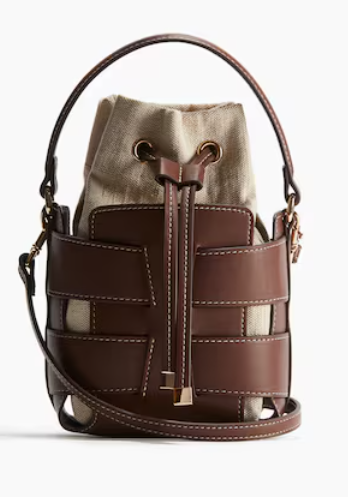
\includegraphics[width=3cm]{70b05981baeb4745ae9906a095701617.png}};
  \end{tikzpicture}}

% ────────────────────────── DOCUMENT ────────────────────────────────────
\begin{document}\pagestyle{empty}

\begin{paracol}{2}
%%%%%%%%%%%%%%%%%%%%%%%%%%%%%%%%%%%%%%%%%%%%
% Colonne GAUCHE (70 %)
%%%%%%%%%%%%%%%%%%%%%%%%%%%%%%%%%%%%%%%%%%%%
{\LARGE\textbf{Judikael MOUROUVIN}}

\bigskip
{\color{maincolor}\Large\textbf{Alternant en marketing digital \& support informatique}}

\medskip
\begin{tabular}{@{}cp{0.45\linewidth}cp{0.45\linewidth}}
  \color{maincolor}\faEnvelope & \href{mailto:jkmou971@gmail.com}{jkmou971@gmail.com} &
  \color{maincolor}\faMapMarker & Route de Cocoyer\;97190 Gosier\\[6pt]
  \color{maincolor}\faPhone & \href{tel:+590 0690 91 14 48}{+590 0690 91 14 48} &
  \color{maincolor}\faLinkedin & \href{}{}
\end{tabular}

\cvsection{EXPERIENCE}

\colorbox{maincolor}{%
  \begin{minipage}{\linewidth}
    \textbf{Alternant en Marketing Digital} \\ Mairie du Gosier – DSI \\ 2023-2024
    \begin{itemize}
      \item Piloté des projets numériques municipaux, assurant leur déploiement dans les délais \item Analysé les besoins des agents et implémenté des solutions digitales adaptées, améliorant leur productivité \item Assuré le support technique et formé les utilisateurs, renforçant l’adoption des nouveaux outils
    \end{itemize}
  \end{minipage}}

\vspace{3mm}


\colorbox{maincolor}{%
  \begin{minipage}{\linewidth}
    \textbf{Animateur de la zone informatique} \\ Pôle emploi, Gosier \\ 2022-2023
    \begin{itemize}
      \item Accompagné quotidiennement les usagers sur les postes informatiques, réduisant les incidents récurrents \item Configuré et entretenu le parc informatique, garantissant sa disponibilité \item Diagnostiqué et résolu les pannes matérielles et logicielles, améliorant le taux de service
    \end{itemize}
  \end{minipage}}

\vspace{3mm}


\colorbox{maincolor}{%
  \begin{minipage}{\linewidth}
    \textbf{Stagiaire informaticien} \\ NUMERIKA, Baie-Mahault \\ 2020-2021
    \begin{itemize}
      \item Installé et maintenu les équipements informatiques du site, sécurisant leur fonctionnement \item Assuré un support de proximité aux collaborateurs, diminuant le temps d’arrêt \item Documenté les procédures de maintenance, facilitant la prise en main des équipements
    \end{itemize}
  \end{minipage}}        % ← générés par build_placeholders()

\cvsection{EDUCATION}

    \begin{tabularx}{\linewidth}{@{}c X@{}}
    \textcolor{sidetext}{\faGraduationCap} &
    \textbf{Bachelor Marketing Digital} \\
    & CFA IUTS \\
    & \begin{itemize}[leftmargin=*]
  \item Acquisition des fondamentaux du marketing en ligne : SEO, SEA, réseaux sociaux \item Gestion de projets digitaux et analyse de performances web
\end{itemize} \\
    & \textit{2023-2024}
    \end{tabularx}
    

\vspace{3mm}


    \begin{tabularx}{\linewidth}{@{}c X@{}}
    \textcolor{sidetext}{\faGraduationCap} &
    \textbf{BTS Système Numérique option Informatique et Réseaux} \\
    & Lycée de Chevalier Saint Georges, Abymes \\
    & \begin{itemize}[leftmargin=*]
  \item Étude des architectures réseaux, systèmes et protocoles \item Pratique de la maintenance matériel et logiciel, support utilisateur
\end{itemize} \\
    & \textit{2019-2021}
    \end{tabularx}
                % ← idem

%%%%%%%%%%%%%%%%%%%%%%%%%%%%%%%%%%%%%%%%%%%%
% Colonne DROITE (30 %)
%%%%%%%%%%%%%%%%%%%%%%%%%%%%%%%%%%%%%%%%%%%%
\switchcolumn

\centering
\roundphoto

\cvsection{SUMMARY}
Professionnel passionné par l’informatique et le marketing digital, je possède une solide expérience en maintenance, support utilisateur et gestion de projets numériques. Mon alternance à la DSI de la Mairie du Gosier m’a permis de consolider mes compétences en déploiement de solutions adaptées et en animation de stratégies digitales. Désormais diplômé d’un Bachelor Marketing Digital, je souhaite mettre mon sens du service et ma rigueur technique au service de nouveaux défis à temps plein.

\cvsection{SKILLS}
\begin{itemize}[leftmargin=*]
\item Administration
\item Maintenance
\item Réseaux
\item Assistance
\item Diagnostic
\item Support
\item Marketing\end{itemize}

\cvsection{LANGUAGES}
\begin{itemize}[leftmargin=*]
\item English - \textcolor{gray}{}
\item Espagnol - \textcolor{gray}{}\end{itemize}

\cvsection{INTERESTS}
\begin{itemize}[leftmargin=*]
\item Lecture \& veille technologique
\item Randonnée / sports outdoor
\item Voyages \& découverte culturelle
\end{itemize}

\end{paracol}
\end{document}
